\documentclass[dvisvgm,tikz]{standalone}
\usepackage{circuitikz}
\begin{document}
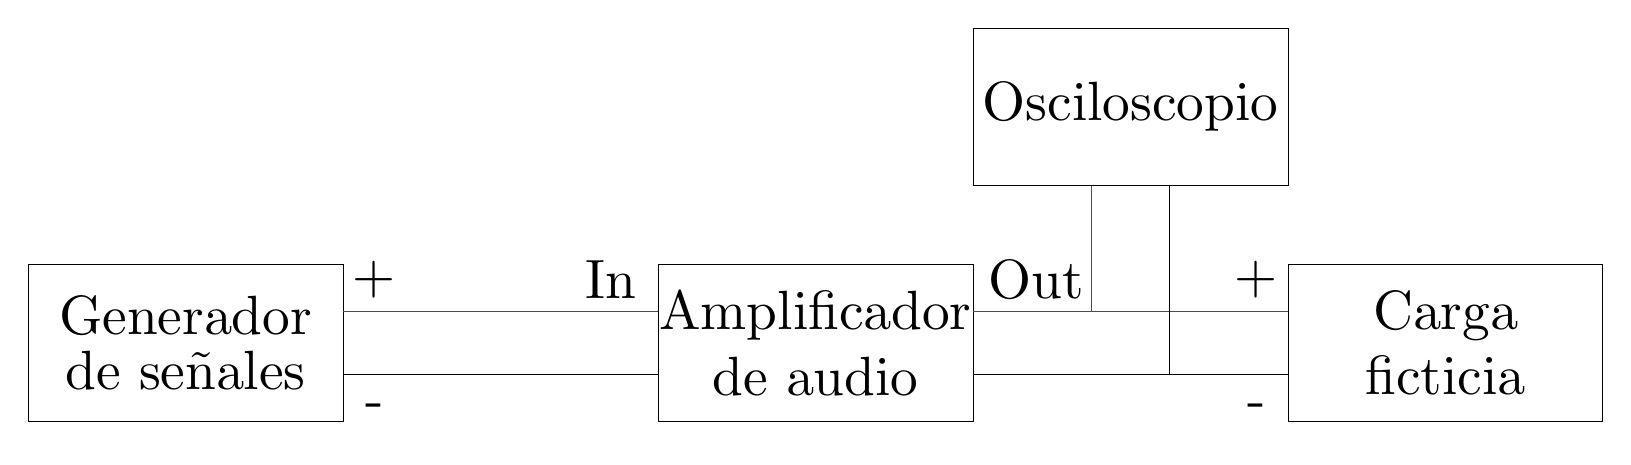
\begin{tikzpicture}[scale=2, every node/.style={transform shape}]
  %\draw[step=0.5,gray,very thin, dotted] (0,0) grid (12,2.5);
  %\draw[step=1.0,gray!50,very thin] (0,0) grid (12,2.5);

  \draw[line width=0.1mm] (1,0) rectangle (3,1) node[pos=.5] {\shortstack{Generador \\ de señales}};
  \draw[line width=0.1mm] (5,0) rectangle (7,1) node[pos=.5] {\shortstack{Amplificador \\ de audio}};
  \draw[line width=0.1mm] (7,2.5) rectangle (9,1.5) node[pos=.5] {Osciloscopio};
  \draw[line width=0.1mm] (9,0) rectangle (11,1) node[pos=.5] {\shortstack{Carga \\ ficticia}};

  \draw[red,   line width=0.1mm] (3.0,0.7) -- (5.0,0.7);
  \draw[black, line width=0.1mm] (3.0,0.3) -- (5.0,0.3);

  \draw[red,   line width=0.1mm] (7.0,0.7) -- (9.0,0.7);
  \draw[black, line width=0.1mm] (7.0,0.3) -- (9.0,0.3);

  \draw[red,   line width=0.1mm] (7.75,0.7) -- (7.75,1.5);
  \draw[black, line width=0.1mm] (8.25,0.3) -- (8.25,1.5);

  \node at (3.2,0.9) {+};
  \node at (3.2,0.1) {-};
  \node at (4.7,0.9) {In};
  \node at (7.4,0.9) {Out};
  \node at (8.8,0.9) {+};
  \node at (8.8,0.1) {-};
\end{tikzpicture}
\end{document}